\chapter{Example Systems} \label{ch:ExampleSystems}
this chapter is all about the actual examples that we've worked through and got an answer for.
It will tie together the VectorEqns and QG chapters and display how we are using the theory to solve problems that might represent physical wave-guides.

\section{Preliminaries}
We should recall the necessary things, such as the definition of the M-matrix, how QG problems work, that now our edges need to be directed as do our derivatives (MB I've used that derivatives INTO the vertex are positive but the opposite convention amounts to multiplying the M-matrix by -1), the vector QG system we are solving, how to build the M-matrix etc.
Also in here should be the general result for the M-matrix column contributions - similar in ilk to EKK paper which should be referenced (again here, if necessary). \newline

Our focus in the examples of this chapter will be to determine the eigenvalues $\omega^2$ of \eqref{eq:CurlCurlEquationDivFree},
\begin{align*}
	-\ktcurl{\ddmes}\bracs{\ktcurl{\ddmes}u} &= \omega^2 u, \quad u\in\ktcurlSobDivFree{\ddom}{\ddmes}.
\end{align*}
Note that in the process we will also determine the eigenfunctions $u$, however these are not the focus of our analysis.
Using the work of chapter \ref{sec:CurlReductionToQG}; we know that we can determine the eigenvalues by solving the quantum graph problem given in \eqref{eq:CurlEdgeEquations}-\eqref{eq:CurlVertexConditions}.
To save on notational clutter we drop the overhead tilde notation for $\widetilde{u}_{2,jk},\widetilde{u}_{3,jk}$ that was used in section \ref{sec:CurlReductionToQG} and also define some convenient constants
\begin{align*}
	\qm_{jk} &= \bracs{R_{jk}\qm}_2, \quad \forall I_{jk}\in E,\\
	\effFreq &= \sqrt{\omega^2 - \wavenumber^2}.
\end{align*}
We also make use of some of the properties of \eqref{eq:CurlEdgeEquations}-\eqref{eq:CurlVertexConditions}.
In particular any (general) solution pair $u_{2,jk},u_{3,jk}$ that solves any two of \eqref{eq:CurlEdgeEquations} necessarily satisfies the remaining equation.
As such we can substitute \eqref{eq:CurlEdgeEquations3} into \eqref{eq:CurlEdgeEquations2} to obtain a single equation in $u_{3,jk}$.
The (general) solution $u_{3,jk}$ that would be obtained from this equation would then allow us to recover $u_{2,jk}$ and satisfy the remaining \eqref{eq:CurlEdgeEquations1}.
Similarly we can also note that a solution pair to \eqref{eq:CurlEdgeEquations} that satisfies \eqref{eq:CurlVertexConditions1}, then satisfies \eqref{eq:CurlVertexConditionsSum2} if and only if it satisfies \eqref{eq:CurlVertexConditionsDeriv}.
Given that our objective is just determining the eigenvalues of \eqref{eq:CurlCurlEquationDivFree}, it is thus sufficient for us to solve the system
\begin{align} \label{eq:QGEquation}
	0 &= -\bracs{\diff{}{t} + i\qm_{jk}}^2 u_{3,jk} + \bracs{\wavenumber^2 - \omega^2}u_{3,jk}.
\end{align}
\begin{subequations} \label{eq:QGVertexConditions}
	\begin{align}
		u_3 &\text{ is continuous at each } v_j\in V, \\
		0 &= \sum_{j\sim k} \bracs{\diff{}{t} + i\qm_{jk}}u_{3,jk}\bracs{v_j}, \quad\forall v_j\in V
	\end{align}
\end{subequations}
for the eigenpairs $\bracs{\omega^2, u_{3,jk}}$.
We shall take the system \eqref{eq:QGEquation}-\eqref{eq:QGVertexConditions} as our starting point for the examples in this section.
In addition, we compute the general form for $u_{3,jk}$ as
\begin{align} \label{eq:CurlEdgeEqnGenSol}
	u_{3,jk} &= e^{-i\qm_{jk}t}\bracs{ C_{+}^{(jk)}e^{-i\effFreq t} + C_{-}^{(jk)}e^{i\effFreq t} },
\end{align}
which will be useful for proving the result of proposition \ref{prop:M-MatrixEntries}. \newline

\tstk{that's all you can write for this section without the quantum graphs section actually having some substance to motivate these objects and this method of solution, guess it's time to start on that!}
\begin{prop}[$M$-matrix entries] \label{prop:M-MatrixEntries}
	Let $\graph=\bracs{V,E}$ be an embedded graph on which the problem \eqref{eq:QGEquation}-\eqref{eq:QGVertexConditions} is posed.
	For each $I_{jk}\in E$ let $\qm_{jk} = \bracs{R_{jk}\qm}_2$ and $l_{jk} = \abs{I_{jk}}$.
	Suppose that $\dmap u = e_k$ where $e_k$ is the $k$\textsuperscript{th} canonical unit vector in $\reals^{\abs{V}}$.
	Then the $j$\textsuperscript{th} entry of $\nmap u$, and hence the $jk$\textsuperscript{th} entry in the $M$-matrix, is given by
	\begin{align*}
		\bracs{\nmap u}_j &= 
		\begin{cases}
			\!\begin{aligned}
				0	
			\end{aligned}			
			& j \not\con k, \\
			\!\begin{aligned}
				-\sum_{j\conLeft k} \effFreq e^{i\qm_{jk}l_{jk}} \csc\bracs{l_{jk}\effFreq} 
				\\ \quad - \sum_{j\conRight k} \effFreq e^{i\qm_{kj}l_{kj}} \csc\bracs{l_{kj}\effFreq}
			\end{aligned}
			& j\neq k, \ j\con k, \\
			\!\begin{aligned}
				\sum_{j\conLeft l} \effFreq\cot\bracs{l_{jl}\effFreq}
				+ \sum_{j\conRight l} \effFreq\cot\bracs{l_{lj}\effFreq}
				\\ \quad - 2\effFreq\sum_{j\conLeft j} \cot\bracs{l_{jj}\effFreq} - \cos\bracs{\qm_{jj}l_{jj}}\csc\bracs{l_{jj}\effFreq}
			\end{aligned}
			& j=k.
		\end{cases}
	\end{align*}
	Note the choice of $j\conLeft j$ in the contributions from loops is simply a convention, $j\conRight j$ is equivalent here.
\end{prop}
\begin{proof}
	The proof is an explicit computation, and follows the same idea as in \tstk{EKK paper result, we just have QM here too} with adjustments for the fact that there are $\wavenumber$ and $\qm$ terms floating around.
	For each $k$, setting $\dmap u = e_k$ provides us with sufficient Dirichlet data at each vertex to eliminate the constants $C^{(jk)}_{\pm}$ in \eqref{eq:CurlEdgeEqnGenSol}.
	This in turn enables us to explicitly write the solutions $u_{3,jk}$, differentiate them, and read off their values at any relevant vertices.
	This then provides us with the value of each term in the sum in $\bracs{\nmap u}_j$, for each $j$.
\end{proof}

\section{The TFR setup but with curls}
As the title says, but make it more formal and fancy and not in reference to the TFR. 
Spectrum is whole real line, because no gaps open...
\begin{figure}[h]
	\centering
	\includegraphics[scale=0.75]{Diagram_TFRGraph.pdf}
	\caption{\label{fig:Diagram_TFRGraph}}
\end{figure}
\begin{figure}[h]
	\centering
	\includegraphics[scale=0.75]{Diagram_TFRQuantumGraph.pdf}
	\caption{\label{fig:Diagram_TFRQuantumGraph}}
\end{figure}

\section{General period cell with lengths system}
the one with the lengths and the annoying result for the determinant.
Play with this to see if any band-gaps emerge :L
\begin{figure}[h]
	\centering
	\includegraphics[scale=0.75]{Diagram_5VertexGraph.pdf}
	\caption{\label{fig:Diagram_5VertexGraph}}
\end{figure}

\section{Thick Vertex Case}
Will need to say ``we can use thick vertices and all remains the same because.." but otherwise then we can give some analysis.
Can include the pretty bandgap plot that I made here :)
\begin{figure}[h]
	\centering
	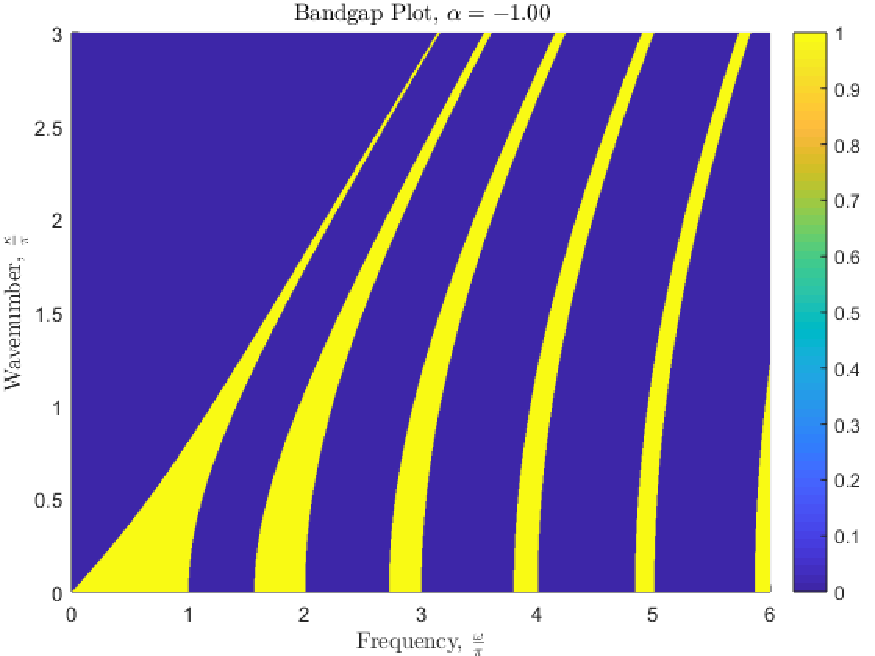
\includegraphics[scale=0.5]{TFR_Curls_BandgapPlot_alpha-1.pdf}
	\caption{\label{fig:TFR_Curls_BandgapPlot_alpha-1}}
\end{figure}

\section{Summary}
Chapter summary of the results and how they might be physically interpreted.
Speculate on future developments.